\chapter{\label{sec:prior_art}Existing Solutions}

The idea of making it easier to interact with low-level hardware from a \gls{PC} is not new. Several solutions to this problem have been developed, each with its own advantages and drawbacks. Some examples will be presented in this chapter.

\section{Raspberry Pi}

\begin{figure}[H]
	\centering
	\begin{subfigure}{.5\textwidth}
		\centering
		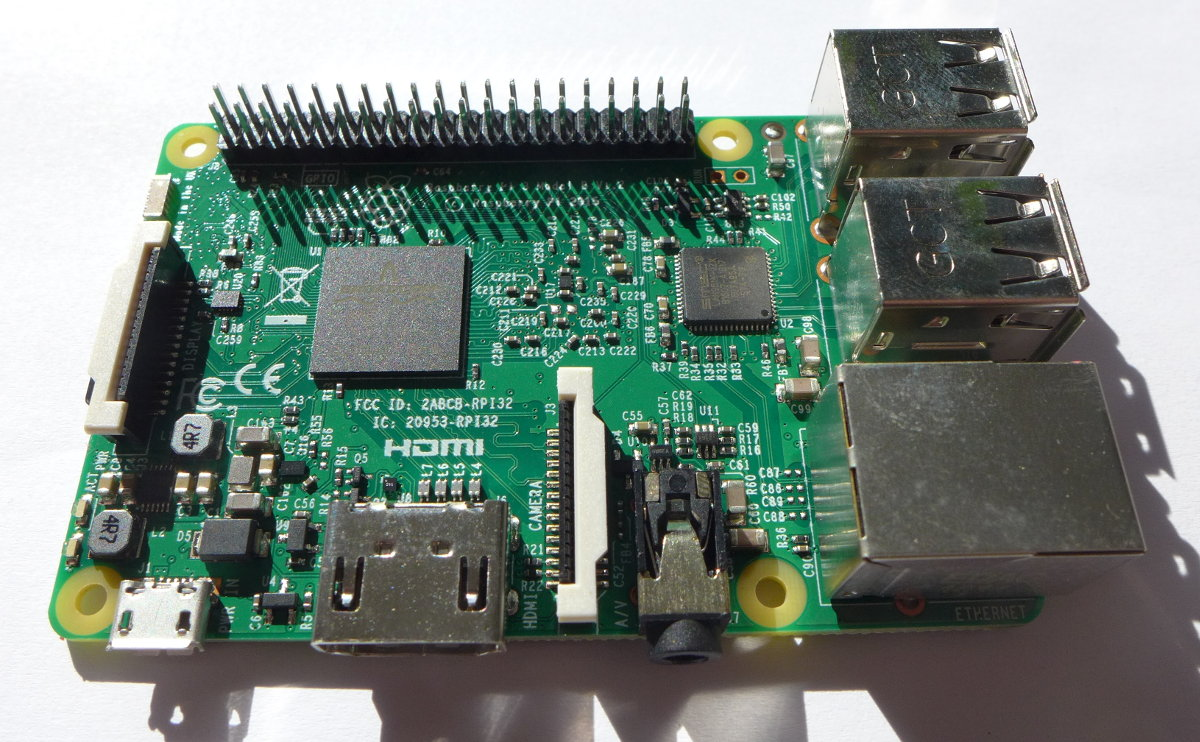
\includegraphics[width=.95\textwidth] {img/pi3-photo.jpg}
		\caption{Raspberry Pi 3 Model B}
	\end{subfigure}%
	\begin{subfigure}{.5\textwidth}
		\centering
		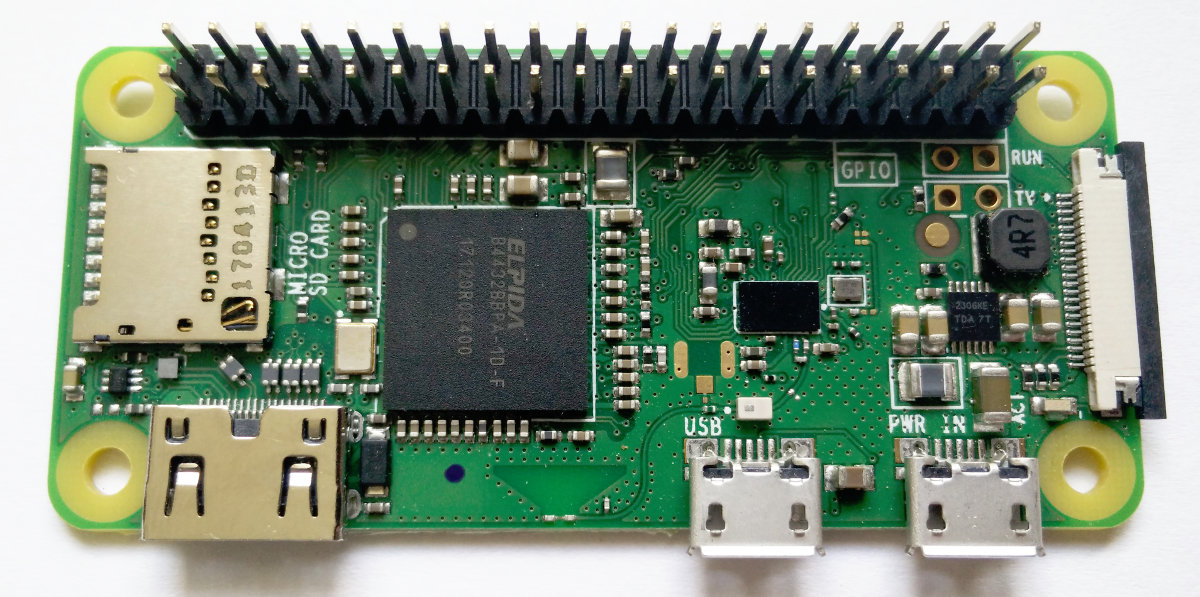
\includegraphics[width=.95\textwidth] {img/pi0.jpg}
		\caption{Raspberry Pi Zero W}
	\end{subfigure}
	\caption{\label{fig:rpi}Raspberry Pi minicomputers}
\end{figure}

The Raspberry Pi (\cref{fig:rpi}) is a low-cost minicomputer targeted at school environments and hobbyists. It is often used for home automation, as a simple web server, or built into projects that take advantage of its powerful processor, such as wildlife camera traps, or data acquisition devices with in-situ processing.

The board's \gls{GPIO} header, a row of pins supporting features such as \gls{SPI}, \gls{I2C}, \gls{UART}, or \gls{PWM}, directly accessible by user applications running on the minicomputer, was one of the inspirations behind GEX.

The Raspberry Pi's functionality clearly overlaps with features we wish to support in GEX. Its processor is powerful enough for a regular \gls{OS} with a graphical user interface, and after attaching a display and a keyboard, it can be used as a \gls{PC}. However, when we have a more powerful computer available and only want to extend it with the \gls{GPIO} header, having to use the Raspberry Pi seems inconvenient; this might be overcome with the use of screen sharing or \gls{SSH}, but a low-complexity solution like GEX certainly has its appeal.

\section{Bus Pirate}

\begin{figure}[H]
	\centering
	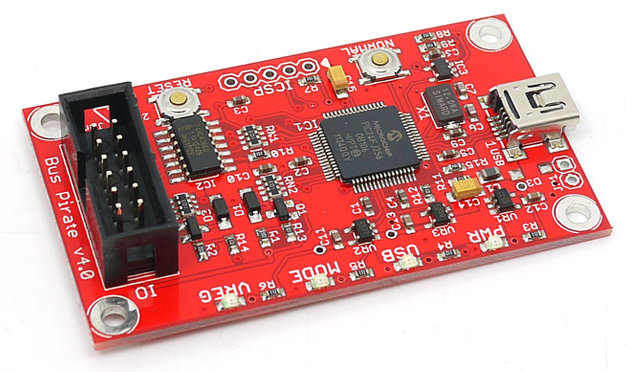
\includegraphics[width=0.5\textwidth] {img/buspirate.jpg}
	\caption{\label{fig:buspirate}Bus Pirate v.4 (photo taken from~\cite{buspirate-product-page})}
\end{figure}

%http://dangerousprototypes.com/blog/about/

% Dangerous Prototypes and manufactured by Seeed Studio\todo{link}
Bus Pirate~\cite{buspirate} is a USB-attached device providing access to hardware interfaces like \gls{SPI}, \gls{I2C}, \gls{USART}, and 1-Wire, as well as features like frequency measurement and direct pin access. The board aims to make it easy for users to familiarize themselves with unknown chips and modules; it also provides a range of programming interfaces to program microcontrollers and memory chips. The board communicates with the \gls{PC} using an FTDI USB-serial adapter.

Bus Pirate is open source and is, in its scope, similar to GEX. It can be scripted and controlled from the PC, connects to USB and provides a wide selection of hardware interfaces.

The board is based on a PIC16 microcontroller running at 32\,MHz. Its \gls{ADC} only has a resolution of 10 bits (1024 levels). There is no \gls{DAC} available on the chip, which makes applications that require a varied output voltage more difficult to implement. Another limitation of the board is its low number of \gls{GPIO} pins, which may be insufficient for certain applications; this, however, is not a hindrance to its main purpose as a bus analyzer and tinkering tool. 

The Bus Pirate is available for purchase at around 30\,USD (at the time of writing), a price comparable to some Raspberry Pi models.

\section{Professional DAQ Modules}

Various professional tools that would fulfill our needs exist on the market, but their high price makes them inaccessible for users with a limited budget, such as hobbyists or students who would like to keep such a device for personal use. An example is the National Instruments \IIC/SPI Interface Device which also includes several \gls{GPIO} lines, their USB DAQ module, or some of the Total Phase \IIC/SPI gadgets (\cref{fig:profidaq}).

The performance GEX can provide may not always match that of those professional tools, but in many cases it will be a sufficient substitute at a fraction of the cost.

\begin{figure}[h]
	\centering
	\begin{subfigure}{.5\textwidth}
		\centering
		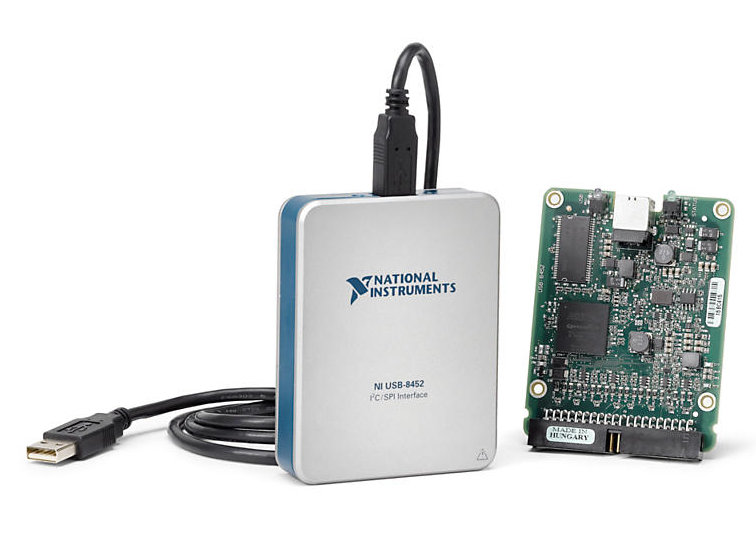
\includegraphics[width=.95\linewidth]{img/ni-i2c-device.jpg}
		\caption{NI \IIC/SPI Interface Device}
	\end{subfigure}%
	\begin{subfigure}{.5\textwidth}
		\centering
		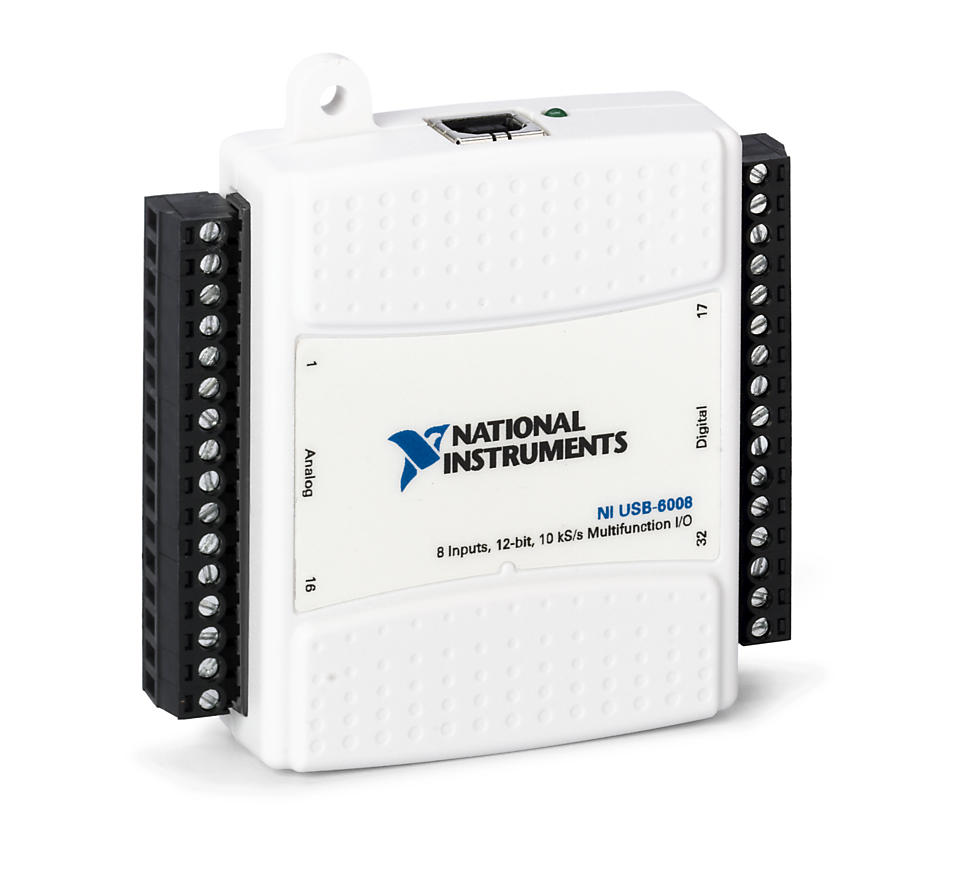
\includegraphics[width=.95\linewidth]{img/nidaq.jpg}
		\caption{NI USB DAQ module}
	\end{subfigure}
	\begin{subfigure}{.5\textwidth}
		\centering
		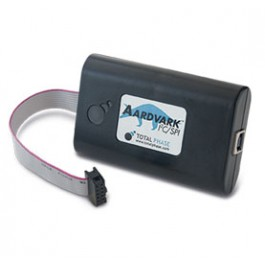
\includegraphics[width=.95\linewidth]{img/total-phase-spi-i2c.jpg}
		\caption{Total Phase SPI/\IIC Host ``Aardwark''}
	\end{subfigure}
	\caption[Professional tools that GEX can replace]{\label{fig:profidaq}An example of professional tools that GEX could replace in less demanding scenarios \textit{(pictures taken from marketing materials:~\cite{nidevice1, nidevice2, tphasedevice})}}
\end{figure}

%http://www.ni.com/en-gb/shop/select/i2c-spi-interface-device}

\iffalse
\section{The Firmata Protocol}

\todo[inline]{links}

Firmata is a communication protocol based on MIDI (\textit{Musical Instrument Digital Interface}) for passing data to and from embedded microcontrollers. MIDI is mainly used for attaching electronic musical instruments, such as synthesizers, keyboards, mixers etc., to each other or to a PC. Firmata was designed for Arduino as a high-level abstraction for its connection to the PC, typically using a FTDI chip or equivalent.

Implementing Firmata in the GEX firmware would make it possible to use existing Firmata libraries on the PC side. However, the protocol is limited by the encompassing MIDI format and is not very flexible.
\fi

